\documentclass[9pt,journal,compsoc]{IEEEtran}
\usepackage[english]{babel}
\usepackage[utf8]{inputenc}
\usepackage{cite}
\usepackage{amsthm}
\usepackage{amsmath}
\usepackage{amssymb}
\usepackage{graphicx}
\usepackage{array}
\usepackage{algorithmic}
\usepackage{url}
\usepackage{subcaption}
\usepackage{float}


% correct bad hyphenation here
\hyphenation{op-tical net-works semi-conduc-tor}

\newtheorem{mydef}{Definition}

\begin{document}

\title{\huge Categorisation of Urban Water Consumptions}

% Author information
\author{
	\IEEEauthorblockN{Joaquim Leitão\IEEEauthorrefmark{1}}
	
	\IEEEauthorblockA{\IEEEauthorrefmark{1}jpleitao@dei.uc.pt \\ CISUC, Department of Informatics Engineering, Univesity of Coimbra, Portugal}
}

% The paper headers
\markboth{Connectivity and Pattern Recognition, 2016-2017}{Connectivity and Pattern Recognition, 2016-2017}


\IEEEtitleabstractindextext{
\begin{abstract}
	The identification and prediction of water consumption patterns plays an essential role in the management of water supply infrastructures, namely in urban environments. Without any accurate prediction or characterisation of the consumptions, water utilities are forced to continuously overestimate water volumes drained to storage tanks, increasing their operation costs and water waste.
	
	The main objective of this work is to identify and locate in time recurrent water consumption patters, featuring a comparative study of popular clustering techniques. Domestic water consumptions for a given region of a median size city, collected during the entire 2016 year, were used in this work.
	
	In the conducted analysis the number of clusters that best fits the data appears to be $4$, covering about three distinct periods of time during the year: The early Summer (June and July), the main Summer months and beginning of Autmn (July, August and September), and the remaining of the year (also with a brief incidence during the previously mentioned months).
	
	Following the adopted and discussed methodology an automatic categorisation of water consumptions is possible without resorting to any sources other than the consumptions dataset. As such, this approach can certainly improve the management of existing water infrstructures, as well as reduce excess water stored in supply storage tanks.	
\end{abstract}

\begin{IEEEkeywords}
	Water Consumption Patterns, Clustering, Time series, Pattern Recognition.
\end{IEEEkeywords}
}


% make the title area
\maketitle
\IEEEdisplaynontitleabstractindextext
\IEEEpeerreviewmaketitle


\IEEEraisesectionheading{\section{Introduction}\label{sec:introduction}}

\IEEEPARstart{I}{n} most cities and urban areas investment in equipment related to water supply and drainage is substantial, being responsible for a considerable share of the budget of many municipalities.

Substantial attention has been given to the construction and installation of new pipe and sewage infrastructures, as well as to maintenance operations on existing infrastructures; however, relatively small efforts have been made to study water consumption patterns in these environments.

Indeed, understanding and accurately predicting such behaviours is extremely important to water companies, as it allows them to improve the management of their infrastructures, namely water storage facilities (such as water tanks and towers): Many water utilities repeatedly overestimate the volume of water needed to supply the population of a given region. Therefore, water companies tend to operate existing water storage tanks close to their full capacity, resulting in higher energy-related costs (since water has to be pumped into the tanks) and in larger volumes of retained water. 

By being capable of characterising water consumption patterns in a given region water companies could adjust water volumes in existing storage tanks\footnote{For obvious reasons this volume must always be overestimated; however, such overestimation could be better controlled.}, improving the management of their finances and reducing excess water volumes retained in storage tanks.

The current work aims at categorising water consumptions in a given region of a median size city, contributing towards an improved understanding and knowledge of water consumption patterns. Therefore, in this work, historic water consumptions are intended to be processed and organised in different groups according to their similarity.

In the field of pattern recognition, tasks of this nature are referred to as \emph{clustering} approaches. Since a time-ordered series of data (water consumptions, in this case) is intended to be processed and clustered, the proposed problem can be considered as \emph{time series clustering}. In this sense, it is important to define this term. We present a definition proposed by Aghabozorgi \emph{et al.} \cite{aghabozorgi2015time}:

\begin{mydef}[Time Series Clustering]
	"Given a dataset of n time series data $D = \{F_{1}, \cdots , F_{n}\}$, time series clustering can be defined as the process of unsupervised partitioning of $D$ into $C = {C_{1}, \cdots , C_{k}}$ in such a way that homogeneous time series are grouped together based on a certain similarity measure."
\end{mydef}

The remainder of this document is organised as follows: Section \ref{objectives} presents the main objectives of this work. In section \ref{dataset_description} water consumption data used in this work is briefly presented. The methodology adopted throughout this work is discussed in section \ref{methodology}. Sections \ref{pre_processing} to \ref{results_assessment} cover the main steps of the work, presented in the methodology section. Finally Section \ref{conclusions} presents a reflection on the work and discussed results, while Section \ref{future_work} covers future research directions.

\section{Objectives}
\label{objectives}

The main objective of the proposed work is related with the categorisation of urban domestic water consumptions in a given region of a median size city.

That is, taking into account information about an entire civil year (from January 1st to December 31st) recurrent consumption patterns must be identified and located in time: an intuitive (and somewhat expected) result is that water consumptions during summer months will have a similar shape, which substantially differs from those recorded during winter months. This could be justified by the fact that many people in that region usually spend summer months away, on vacation.

In this sense, the appropriate steps of a pattern recognition system will be considered, namely: (i) data pre-processing; (ii) pattern recognition techniques - in this case clustering techniques; (iii) analysis of the experimental results.

\section{Dataset Description}
\label{dataset_description}

The dataset to be used in the proposed project contains domestic water consumptions in different regions of a median size city. The available data corresponds to the entire 2016 year and was generated as a result of a collaboration with \emph{Águas de Coimbra}\footnote{\url{http://www.aguasdecoimbra.pt/}}, the public water company in the city of Coimbra, Portgual.

In a real scenario water consumption's measurement is carried out in strategic locations of the city, through measurement and control zones - \emph{ZMC}\footnote{Or in portuguese, \emph{Zonas de Medição e Controlo}.}. These infrastructures provide a more efficient management of the water distribution systems, enabling the network's management in logical zones of analysis and allowing the adoption of measures to control water losses.

Collected data corresponds to a time series of total water volume distributed to the region in question - recorded as a floating point number whose units are $m^{3}/h$. Therefore, pairs of values $(time, volume)$ are provided. The collection time is provided in the format \emph{dd/mm/yyyy HH:MM:SS}.

During the data acquisition equipment errors and malfunctions can occur, resulting in the failure to record the total consumptions. In such moments, a value of \emph{"n/a"} is presented for the total distributed water volume, signalling the missing value. The developed pattern recognition system must adopt proper techniques to deal with these missing values.

\section{Methodology}
\label{methodology}

Extensive research has been made in the field of time series clustering, resulting in the adoption and proposal of a wide variety of clustering approaches and techniques. In a 2015 survey on time series clustering, Aghabozorgi \emph{et al.} \cite{aghabozorgi2015time} highlights techniques such as \emph{hierarchical clustering}, \emph{k-means clustering} and \emph{k-medoids clustering}. Other techniques have also been applied, such as neural networks and variations of the mentioned algorithms, namely of \emph{k-means} ans \emph{k-medoids}.

Determining the most appropriate technique to be applied in our problem is far from being an easy task. The same methods applied on data of distinct natures can produce completely different results, and the same can even occur with similar data, collected from distinct sources and (most probably) with a different process.

As a result, in the current work, different techniques are intended to be explored in an attempt to determine the ones that appear to be more suitable to the collected data. These techniques fall in four distinct categories that compose four main steps of time series clustering. In subsequent sections a more derailed overview of such categories will be provided.

\begin{enumerate}
	\item \textbf{Time Series pre-processing}, comprising two major tasks: computing the unit of analysis for the time series; and imputing missing values
	
	\item \textbf{Time Series Representation}, consisting in the application of dimensionality reduction techniques. As will be explained later in this section, both raw time series data and dimensionality reduced time series data is intended to be clustered, in order to compare the results obtained with both methods.
	
	\item \textbf{Time Series Segmentation}, consisting in the application of clustering techniques to group similar samples together.
	
	\item \textbf{Results analysis and assessment}
\end{enumerate}
 
Regarding missing data imputation, three distinct techniques are considered to be applied to provide sounding estimations for missing water consumptions data: fitting a polynomial expression, fitting an ARIMA model or the application of Kalman Filters.

With respect to time series representation methods, two alternatives are intended to be considered: on one side, the popular \emph{raw time series} representation - where time series are represented as an ordered list of values collected over time; as an alternative, the applications of dimensionality reduction methods via \emph{Principal Components Analysis} and \emph{Stacked Autoencoders} is also explored.
	
Several clustering algorithms have been proposed and studied in the literature; however, based on the studied and referenced works, more traditional algorithms such as \emph{Hierarchical} and \emph{K-Means} clustering still remain popular and valid choices among researchers in this field. In this sense, their performance when applied to our data will be assessed. Another algorithm applied in time series clustering problems will be implemented and evaluated: this is the case of the recently proposed \emph{TADPole} density-based clustering algorithm, featuring a pruning strategy that softens the computational burden of the application of traditional clustering algorithms to time series.

\section{Time Series Pre-Processing}
\label{pre_processing}

As stated in section \ref{methodology}, time series pre-processing comprises two main iterations: computing the unit of analysis of the time series and imputing missing values in time series' readings. These steps will be covered in more detail in their own subsections.

\subsection{Unit of Analysis}

When identifying patterns of recurrent behaviour in time series data it is important to determine the periods of time with the higher contributions to the overall signal. In other words, the most intense and important periods of time are sought.

Similarly to the works of Abreu \emph{et al.}\cite{abreu2012using} and Calabrese \emph{et al.}\cite{calabrese2010eigenplaces}, a \emph{Fourier} analysis can be conducted on the collected time series data to determine the frequencies with higher contribution. In this sense, a \emph{Fast Fourier  Transform} (FFT) was performed on the time series data. 

Analysing the results of such transformation, it was determined that the frequency with the largest contribution to the resulting signal was the frequency 0 $Hz$. Even though this may seem an unexpected result, a valid explanation can be found: by performing the FFT of a given signal, the frequency with higher contribution is usually an approximation of the fundamental frequency. As the signal being analysed (the time series data) is not periodic, its fundamental period is infinite, rendering its fundamental frequency to be 0 $Hz$. In such scenarios, the second frequency with higher contribution is usually considered as the unit of analysis. In this case such a frequency was around $24h$, suggesting this to be the unit of analysis.

With this finding, an aggregation of the time series values was conducted: the values of the original time series were recorded with a one-minute interval; since the unit of analysis is $24h$, each sample to be clustered contains readings of one day, with an interval of $1h$\footnote{Therefore, each sample consists in a list of 24 values, one per hour. These individual hourly consumptions were obtained simply by adding all partial consumptions in the same hour.}.

\subsection{Missing Data Imputation}

In almost all real-life applications, errors in the data collection procedures are prompted to occur, forcing data analysis and processing methods to properly deal with missing and invalid values. Substantial research has been performed on the topic of missing data imputation, resulting in different methods and techniques being proposed and tested in a variety of problems.

Nevertheless, choosing a valid missing data imputation technique to be applied in a given problem is far from being an easy task. The same method can have completely distinct performances when applied to different data, of diverse natures and/or collected in different ways. In the particular case of this work, no previous studies of the performance of missing data imputation methods had been conducted on the collected data. As a result, a choice was made to browse the literature on this topic and test the application of the most cited and used ones in the collected data.

Steffen \emph{et al.}\cite{moritz2015comparison} studied the application of different missing data imputation methods on univariate time series. In their work, the authors obtained interesting results for approaches exploring linear interpolation, ARIMA and SARIMA models and Kalman Filters. 

Alternative methods can also be considered. Usually more active in time series prediction and classification, techniques featuring artificial neural networks, decision tress or k-nearest neighbours\cite{troyanskaya2001missing, yu2014short} can also be applied to compute estimations for missing values. In addition, traditional time series analysis methods such as autocorrelation and trend analysis have also been applied\cite{abreu2012using}, as well as expectation-maximization and multivariate algorithms on lagged data\cite{moritz2015comparison}.

Inspired by the results reported on the literature, and after an initial study of the different methods, a choice was made to select the following three missing data imputation methods for further analysis: (i) linear interpolation; (ii) ARIMA; (iii) Kalman Filter.

At this point, the goal of this analysis was to study the performance of these methods when applied to the collected data. This study was conducted as follows: Initially individual samples were divided into samples that contained missing values and samples without missing value\footnote{The reader must keep in mind that individual samples consist in a list with water consumptions for a given day, featuring hourly values.}. For each complete sample missing values were artificially introduced. Each method was then applied to the individual samples and the correctness of their imputations was assessed using the \emph{root mean squared error} (rmse) metric.

Overall the Kalman Filter produced better estimates than the competing alternatives: An average rmse of about $263.83$ was registered (against a rmse of about $571.37$ for the ARIMA model and $12403.17$ for the linear interpolation), and the Kalman filter produced better daily estimates (smaller rmse on individual samples) in 189 days (against 72 for the ARIMA model and only 4 for the linear interpolation).

Based on such results the Kalman Filter was chosen as the imputation approach for our data. Therefore, for each day where missing data were registered, a Kalman Filter model was computed and estimations for the missing data in that day were obtained.

\section{Time Series Representation}
\label{time_series_representation}

When working with high dimensional data, computational requirements grow both in terms of memory and execution time: if each time series contains more values then it will require more space in memory and, therefore, if a larger number of time series is intended to be clustered or processed in some way, substantially more memory may be required to load all the time series data. In addition, specially in the case of clustering, distance computation between data samples is often performed; if a larger number of samples is considered, each comprising several dimensions, distance computation between pairs of samples will take longer to compute, as will the overall process.

Another motivation for seeking alternative time series representations, as pointed out by Aghabozorgi \emph{et al.}\cite{aghabozorgi2015time}, has to do with the fact that when measuring the distance between raw time series samples highly unintuitive results may be gathered resulting in the clustering of series similar in noise, instead of shape. It must be noticed that the adopted distance metric tends to highly influence the clustering results.

In this sense, several time series representation methods have been proposed in the literature. Aghabozorgi \emph{et al.} presents a taxonomy comprising four main categories: i) Data adaptive; (ii) Non-data adaptive; (iii) Model-based; and (iv) Data dictated. The choice of time series representation has a big impact in the outcome of the clustering exercise, in both quality and execution time. Furthermore, time series representation also affects the choice of distance metric (also called dissimilarity function).

In the specific clustering problem being tackled in this work, where time series containing similar behaviours are intended to be grouped together, one of the major challenges to be faced has to do with the dissimilarity function (that is, how to determine that two time series are close together). Even though it is computationally expensive, the \emph{Dynamic Time Warping} (DTW)\cite{chu2002iterative} distance metric is quite popular, having been extensively adopted when dealing with raw time series data\cite{liao2005clustering, petitjean2014dynamic, izakian2015fuzzy, aghabozorgi2015time} and being considered a more robust distance metric for time series\cite{wang2013experimental}. 

As the DTW targets time sequences, it can be concluded that a substantial number of approaches adopt a raw time series representation. Dimensionality Reduction (DR) techniques such as \emph{Principal Components Analysis} (PCA) have also been explored \cite{abreu2012using} in an attempt to represent time series samples in fewer dimensions, thus reducing the computational burden of distance computation. As the application of DR techniques loses the temporal sequence of the data, alternative distance metrics need to be considered.

In light of the discussion carried out in this section, in the scope of the current work, it is intended to explore clustering performance obtained using two distinct time series representation approaches: (i) \textbf{Raw time series representation}, featuring the use of the popular \emph{Dynamic Time Warping} distance metric; (ii) \textbf{"Dimensionality-Reduced" time series representation}, featuring the use of the classical \emph{Euclidean} distance.

\subsection{Raw Time Series Representation}

With respect to the \emph{raw} time series representation not much needs to be added to what has already been mentioned. Initially, this representation can be seen as considering raw collected time series values.

Taking into account the pre-processing steps mentioned in section \ref{pre_processing}, imputed time series corresponding to daily lists of hourly water consumption readings should be considered at this point; however, an additional step must be considered: when working with raw time series data, performing a \emph{Z-Normalization} of the data can significantly improve distance computation results with the DTW metric\cite{mueen2016extracting}.

As a result, when working with raw time series representation, a \emph{Z-Normalization} of the data was conducted. The \emph{Z-Normalization} can be defined as:

$$X = \frac{X - MEAN(X)}{STD(X)} $$

\subsection{Dimensionality Reduction for Time Series}

Regarding the application of dimensionality reduction techniques to time series data, two popular algorithms of this nature were compared: \emph{PCA} and \emph{Stacked Autoencoders} (SAEs). The comparison was based on the rmse on reconstruction and on visual inspection of the reconstructed series.

In PCA the target number of features was selected as a function of the percentage of explained data variance. In this sense, principal components capable of representing $90\%$ of the data variance were selected, yielding a reduced dimensionality of 3 features.

SAEs were then trained for dimensionality reduction, targeting the same number of features as PCA. Different network architectures were considered while training the SAEs (that is, different number of autoencoders with different numbers of neurons per hidden layer, different activation functions, etc); however, in the best scenarios, SAEs were only capable of getting close to PCA in terms of reconstruction error, producing reconstructed time series considerably more distant to the original ones than PCA.

It is also worth mentioning at this point that both PCA and SAEs approaches were tested with normalised data, using the \emph{Min-Max} method. Figure \ref{day3_reconstruction} presents a reconstruction of water consumptions for one day using both a PCA decomposition and Stacked Autoencoders.

\begin{figure}[ht]
	\centering
	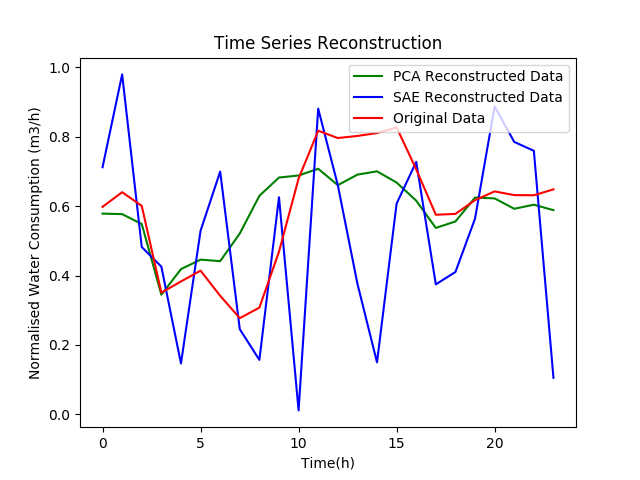
\includegraphics[scale=0.5]{images/pca_sae_day3.png}
	\caption{Reconstruction of water consumptions for one day using a PCA decomposition and a Stacked Autoencoder.}
	\label{day3_reconstruction}
\end{figure}

From the analysis of figure \ref{day3_reconstruction} it is clear that, even though SAEs may be able to reconstruct the original data with an error close to PCA, SAEs fail in capturing the shape and tendency of the series. As a proper learning could not be obtained with SAEs, PCA was the dimensionality reduction technique chosen to be applied in the experiments and exercises carried out in the remainder of this work.

\section{Clustering}

The choice of which clustering algorithm to apply in a given problem can strongly condition the obtained results. Several clustering algorithms have been proposed over the years and applied to a wide variety of problems.

It is common among authors to characterise and classify clustering approaches according to how the algorithms work. Aghabozorgi \emph{et al.}\cite{aghabozorgi2015time} proposes a general categorisation of clustering algorithms applied to time series featuring six different groups: Hierarchical, Partitioning, Model-based, Density-based, Grid-based and Multi-step clustering.

As mentioned in section \ref{methodology}, from the conducted literature review on time series clustering \emph{Hierarchical} and \emph{K-Means} clustering algorithms were identified as the most popular choice among researchers.

One of the main drawbacks of most time series clustering algorithms is related with the computational burden of finding similarities in the data being clustered. As the most robust similarity measures for time series rely on a raw representation, continuously searching for patterns based on similarities/dissimilarities in the data becomes very expensive in computation time.

Motivated by the fact that robust and less demanding alternatives to metrics such as the \emph{DTW} have not been achieved, some researchers studied ways of reducing this computational burden. This is the case of \emph{TADPole}\cite{begum2015accelerating}. Proposed in 2015 by Begum \emph{et al.}, TADPole exploits upper and lower bounds on DTW in a novel pruning strategy that avoids a large fraction of distance calculations, achieving results identical to brute force (but at least an order of magnitude faster).

In this sense, the mentioned cluster algorithms were selected for analysis at this point. Regarding HC and K-Means, as is often performed in the literature, both algorithms were combined\cite{jain2010data}. In the remainder of this section, details regarding the implementation and experimental setup of the two sets of algorithms being compared are covered.

\subsection{Combining Hierarchical and K-Means Clustering}

Formulating K-Means clustering into an algorithm comprises quite simple steps. Nevertheless, this simplicity does not avoid some of the most well-known and documented drawbacks of this algorithm: K-means requires the specification of a number of clusters prior to its execution; resulting from the previous point, K-means always groups the data into the specified number of clusters, meaning even if the number of clusters is inadequate to the dataset at hand, K-means will find such a number of partitions; even on perfect datasets it can get stuck on local minimum; and lastly, the final clustering solution is very sensitive to the initial cluster selection.

To avoid (or at least soften) these problems, an hybrid approach is typically used by combining \emph{hierarchical clustering} and \emph{k-means} methods. The procedure is as follows:

\begin{enumerate}
	\item Compute hierarchical clustering and cut the resulting dendrogram into k-clusters.
	
	\item Compute the centroid of each cluster.
	
	\item Compute K-means by using the previously computed centroids as the initial cluster selection.
\end{enumerate}

\subsection{Centroid Computation in K-Means}

Besides specifying the number of clusters, K-Means also allows for different methods to be applied when computing the centroid representative of a given cluster. A widely used method that can be applied to many distance metrics involves computing, for each dimension of the data, the average of all the samples assigned to the cluster in question. For this reason this method is often referred to as the \emph{average} method.

As mentioned by Aghabozorgi \emph{et al.}\cite{aghabozorgi2015time}, when working with time series data the average centroid computation method tends to only be applied when time series have equal length and a none-elastic distance metric (such as the Euclidean distance) is employed.

When time series are allowed to have different lengths, or when distance metrics of other natures are employed (namely the DTW) simply performing the mean of the time series at each point can fail to capture the average shape of all the time series in the given cluster. As a result, alternative centroid computation methods more adequate to these distance metrics have been studied.

Probably the most common centroid computation method used with raw time series data is the \emph{medoid} method. According to this method, the centroid is the sample that minimizes the sum of squared distances to all the other samples within the cluster. Examples of the application of this method can be found in \cite{liao2006adaptive, izakian2015fuzzy}.

A more recent centroid computation method is the \emph{DTW Barycenter Averaging} (DBA)\cite{petitjean2011global}, proposed in 2011 by Petitjean \emph{et al.}. This method was specified for the DTW distance metric and, according to the authors of the cited work, is claimed to outperform all existing averaging techniques when applied to datasets of the UCR Archive\cite{keogh2006ucr}.

When computing the cluster centroid, DBA tries to minimize the sum of squared DTW distances from the average sequence (that is, the centroid) to all the sequences assigned to the cluster in question. A local optimisation strategy is implemented, which strongly depends on an initial guess for the average sequence - the initial centroid guess. As a result, improved results are usually obtained by performing multiple random initial starts. An example study making use of the DBA to compute the centroids for K-Means clustering can be found in \cite{petitjean2014dynamic}.

In short, taking into account that two distinct time series representation techniques are intended to be applied, different centroid computation methods were also implemented and the performances of the resulting clusterings compared:

\begin{itemize}
	\item Regarding the \emph{DTW} distance metric, the following centroid computation methods were considered: \emph{Average}, \emph{Medoid} and \emph{DBA}.
	
	\item With respect to the \emph{Euclidean} distance metric, only the \emph{Average} centroid method was considered.
\end{itemize}

\subsection{TADPole}

In the beginning of the current section a brief introduction to the TADPole clustering algorithm was performed, highlighting its main characteristics and motivations leading to its development. Regarding implementation details of this algorithm, two parameters must be defined prior to its applications: the \emph{window size} used in the DTW computations and a \emph{cutoff distance}.

The TADPole algorithm makes use of a centred window (of size $w$) when computing distances (using the DTW metric). For any observation $x_{i}$ the algorithm considers the points in the range $x_{i-w}$ and $x_{i+w}$ in the DTW computation. As such taking into account that the DTW is only applied for raw time series representation, and that such time series have a dimensionality of $24$, a window size of $23$ was defined.

The second parameter that needs to be defined is the cutoff distance, often represented as $d_{c}$. In an initial step of the algorithm, upper and lower bound on the DTW are used to find time series with many close neighbours. The mentioned cutoff distance is used as a threshold when determining a time series' neighbours: Any other time series whose distance is below $d_{c}$ is considered a neighbour. In the current work initial experiments were performed with different values for the $d_{c}$ threshold, obtaining a value of $1.5$ as the outcome. Nevertheless, further research on the most appropriate and adequate value for this parameter can still be performed.

Finally, regarding the cluster computation, TADPole takes the series that lie in dense areas (that is, the series that have many neighbours) as the cluster centroids.

\section{Results Assessment}
\label{results_assessment}

The current section covers the distinct experiments conducted in the course of this work, presenting and discussing its main findings. As acknowledged in the previous section, different configurations for the clustering process were defined. Overall, the experimental procedure and consequent results analysis can be summarised in four main steps:

\begin{enumerate}
	\item Initially estimates for the number of clusters were obtained by performing \emph{Hierarchical Clustering} on the time series data and analysing the obtain dendrogram.
	
	\item Apply an hybrid clustering algorithm, where the centroids obtained for the different selected number of clusters in the previous point are used as initial centroids for the \emph{K-Means Clustering} algorithm.
	
	\item Apply cluster evaluation metrics to assess the quality of the clusters computed in the hybrid approach.
	
	\item Based on the cluster quality computed in the previous point select a subset of clustering results to be further analysed. Analysis conducted at this point focuses on descriptive characteristics of the categorisation performed, namely percentage of weekdays and weekend-days assigned to each cluster, percentage of days of each month assigned to each cluster, among others.
\end{enumerate}

In this sense, each of the four points mentioned in the previous listing will be covered in a separate subsection, within the remainder of the current section.

\subsection{Initial Number of Cluster Estimates}
\label{initial_number_clusters}

Based on the experimental setup presented in table \ref{experiments_summary_table}, and discussed throughout the document, time series' similarities were computed based on two distinct distance metrics: DTW and Euclidean. As such, hierarchical clustering using both metrics was computed to obtain the initial estimates for the number of clusters. Figures \ref{hierarchical_clustering_dtw} and \ref{hierarchical_clustering_euclidean} present the dendrograms obtained:

\begin{figure}[ht]
	\centering
	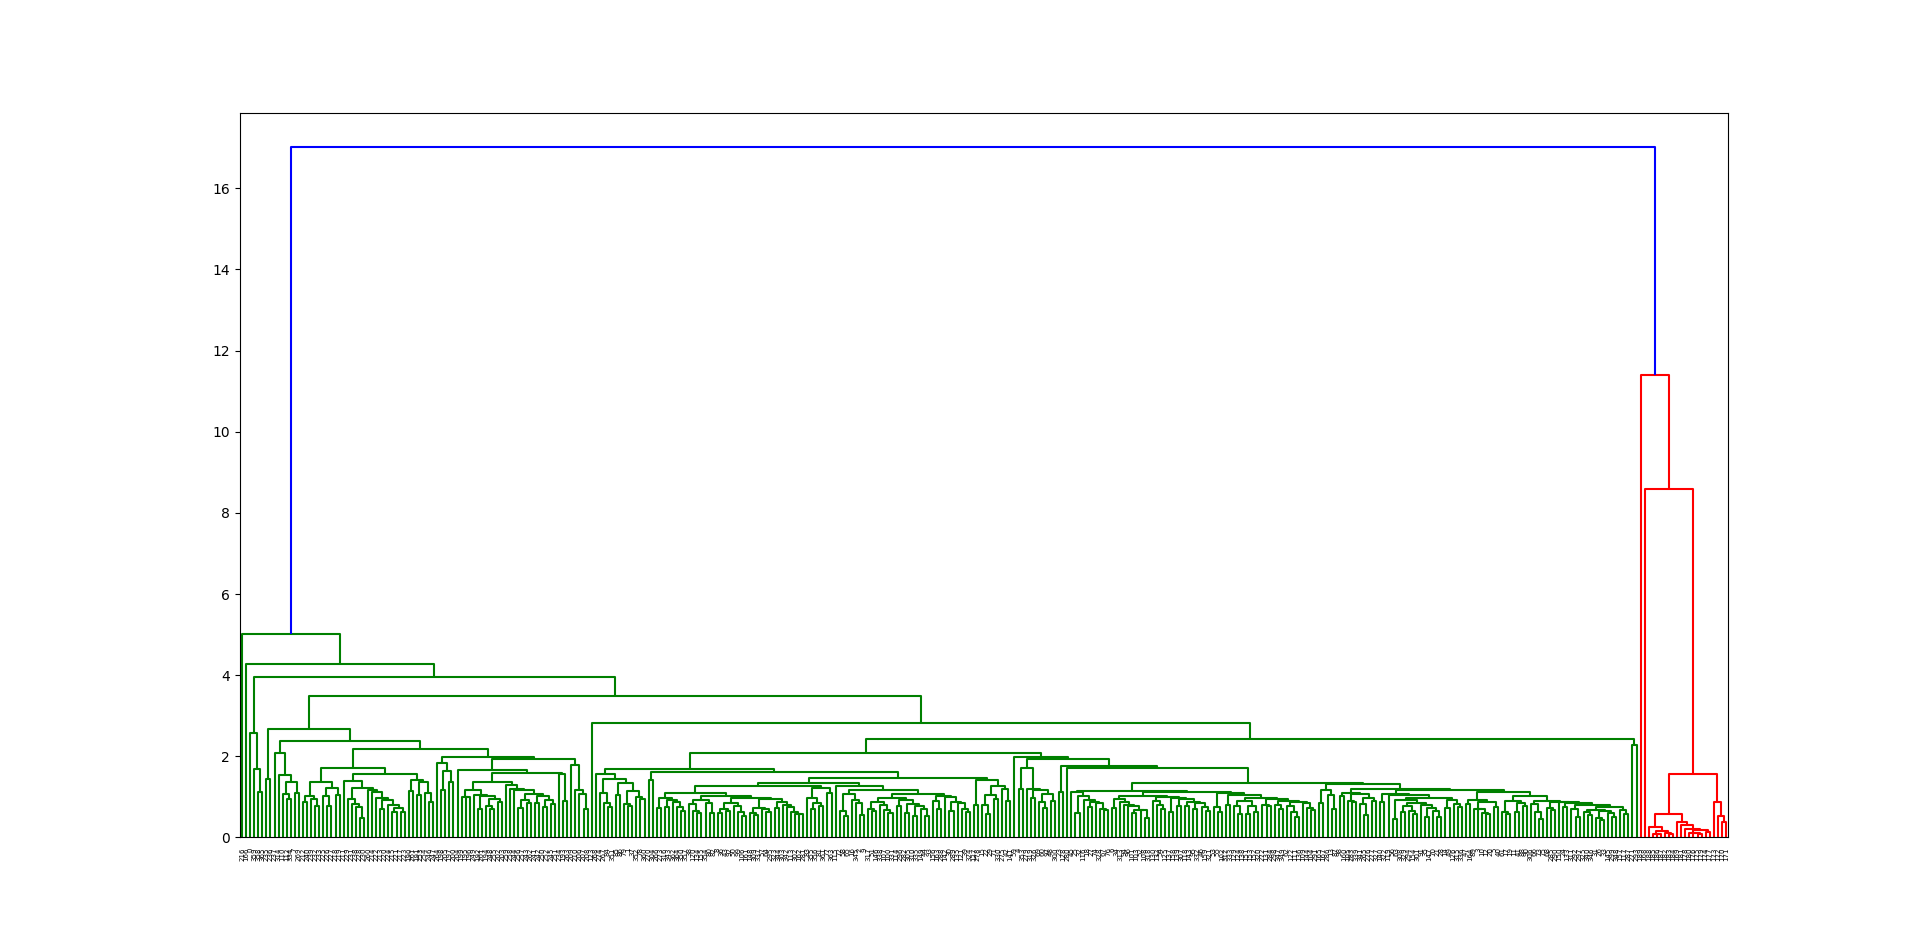
\includegraphics[scale=0.2]{images/Hierarchical_Clustering_DTW.png}
	\caption{Dendrogram obtained using the DTW metric.}
	\label{hierarchical_clustering_dtw}
\end{figure}

Starting with the analysis of Figure \ref{hierarchical_clustering_dtw}, referring to the hierarchical clustering of the z-normalised time series data, 2 major and uneven clusters can be identified and further analysed.

With respect to the right side of the dendrogram (represented in red) three main clusters appear to form. Further divisions can only be considered for significantly smaller distances, for which a high number of clusters needs to be considered. Analysing the left side of the dendrogram (represented in green) several divisions can be identified. For distances smaller than about 3 a high number of divisions can be identified.

Since water consumption patterns for an entire year are intended to be discovered with the goal of improving urban water management, the target number of clusters does not need to be considerably high: for example, if 300 clusters were formed it would be impossible to identify recurrent patterns of consumption.

In this sense, and considering the high number of divisions identified at the mentioned distance, a decision was made to keep it as the maximum number of clusters considered in this work. As the identified number of clusters for the mentioned distance is 8, the K-Means clustering algorithm will be applied to time series data using the DTW metric for a target number of clusters from 2 to 8. The reader's attention is drawn to Table \ref{experiments_summary_table}, where this range is presented.

\begin{figure}[ht]
	\centering
	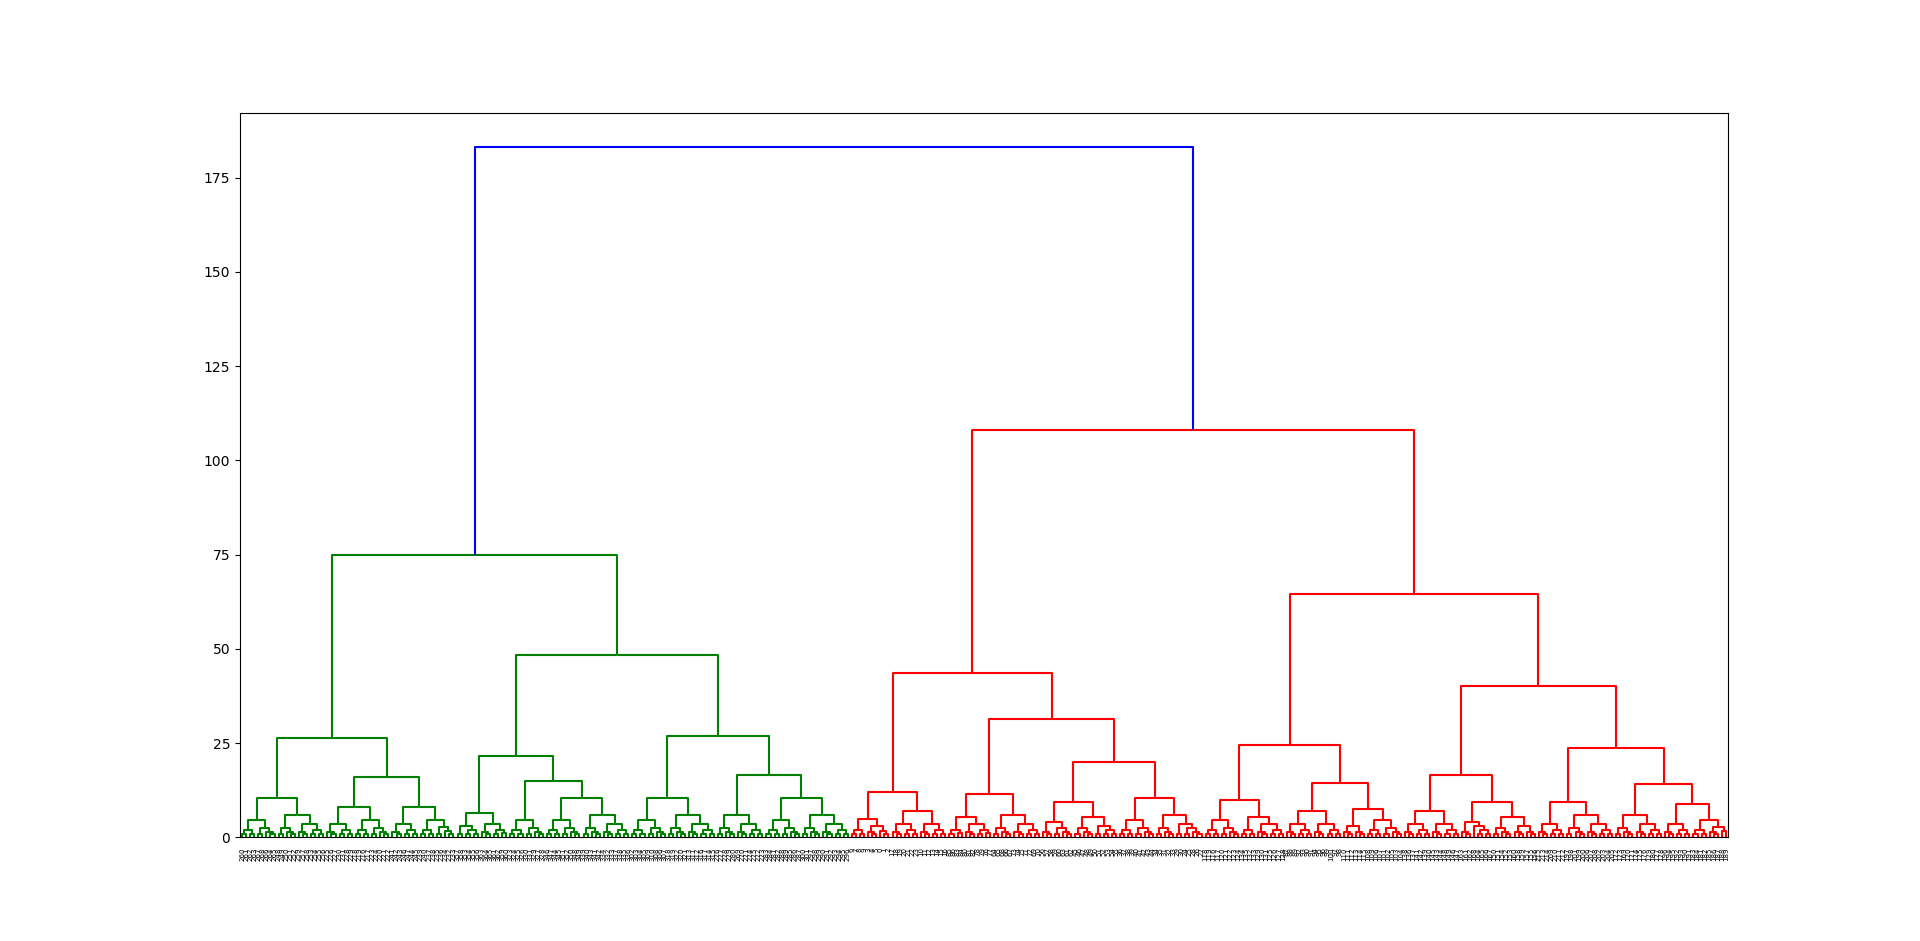
\includegraphics[scale=0.18]{images/Hierarchical_Clustering_Euclidean.png}
	\caption{Dendrogram obtained using the Euclidean metric.}
	\label{hierarchical_clustering_euclidean}
\end{figure}

Moving on to time series data represented using dimensionality reduction techniques the scenario is different from the one presented in Figure \ref{hierarchical_clustering_dtw}: even though two main clusters can still be identified, they are not as unbalanced as the ones in the previous analysis.

By using a reasoning similar to the previous analysis, for distances lower than 50 the number of clusters begins to increase rapidly, suggesting that distance to be defined as the limit for the number of clusters which, is this case, is 8. Similarly to the previous analysis, this value is presented in Table \ref{experiments_summary_table}.

Being in a completely unsupervised scenario alternative ranges for the number of clusters could be considered. Furthermore, a cyclic process could even be considered in which the dendrogram would be initially analysed to extract estimates for the clusters, which would be computed using the K-Means algorithm. Upon further analysis of the results obtained with the K-Means the dendrogram could be analysed again, and new estimates could be computed, repeating this process. Nevertheless, and because of time restrictions, this process was only performed once.

\subsection{Summary of the Experiments}
\label{experiments_summary}

Following the discussion started in the previous sections, Table \ref{experiments_summary_table} presents a summary of the experiments performed, mentioning the algorithms and respective configurations adopted.

\begin{table}[ht]
	\centering
	\caption{Summary of the experiments performed.}
	\label{experiments_summary_table}
	\begin{tabular}{|c|c|c|c|c|}
		\hline
		Data Type                                               & \begin{tabular}[c]{@{}c@{}}Distance\\ Metric\end{tabular} & \begin{tabular}[c]{@{}c@{}}Clustering\\ Algorithm\end{tabular} & \begin{tabular}[c]{@{}c@{}}Centroid\\ Computation\end{tabular}   & \begin{tabular}[c]{@{}c@{}}Number of\\ Clusters\end{tabular} \\ \hline
		Raw                                                     & DTW                                                       & \begin{tabular}[c]{@{}c@{}}HC\\ +\\ K-Means\end{tabular}       & \begin{tabular}[c]{@{}c@{}}Average;\\ DBA;\\ Medoid\end{tabular} & 2 to 8                                                       \\ \hline
		\begin{tabular}[c]{@{}c@{}}Reduced\\ (PCA)\end{tabular} & Euclidean                                                 & \begin{tabular}[c]{@{}c@{}}HC\\ +\\ K-Means\end{tabular}       & Average                                                          & 2 to 8                                                       \\ \hline
		Raw                                                     & DTW                                                       & TADPole                                                        & -                                                                & 2 to 8                                                       \\ \hline
	\end{tabular}
\end{table}


\subsection{Initial Results Analysis}

After obtaining the initial estimations for the clusters the segmentation of the water consumptions must be performed. As discussed throughout the document, approaches of different natures are intended to be compared, raising the need to define metrics that assess the quality of the computed clusters, thus allowing the comparison of the different approaches.

Evaluating algorithms' performance in unsupervised problems such as clustering (without knowing the optimal number of clusters and assignments of each sample) is a challenging task and still considered an open research problem\cite{aghabozorgi2015time}, mostly because of the ambiguity and subjectiveness underlining the definition of a cluster.

Popular evaluation metrics involve \emph{internal} indexes, where cluster quality is summarised to a single score without resorting to any externally supplied labels or ground truth. Whenever such information is available \emph{external} indexes may be applied. In the current work, a completely unsupervised scenario is faced, calling for the application of \emph{internal} indexes.

Several internal indexes have been proposed in the literature to assess cluster quality. In the current work the following were considered:

\begin{itemize}
	\item \emph{Silhouette Coefficient} (SC), also referred to as silhouette index, score or value. SC measures how similar a sample is to others in its own cluster in comparison to other clusters. It is defined as the average of individual samples' silhouette values, $s(i)$, computed as:
	
	$$s(i) = \frac{b(i) - a(i)}{max\{b(i); a(i)\}} $$
	
	where $a(i)$ is the average dissimilarity of sample $i$ to all samples in the same cluster and $b(i)$ is the lowest average dissimilarity of sample $i$ to any other cluster. SC takes a value in the range $[-1, 1]$ where values closer to $1$ suggest more dense and well-separated clusters.
	
	\vspace{0.3cm}
	
	\item \emph{Calinski-Herabaz Index} (CH), also referred to as the \emph{Variance Ratio Criterion} (VRC). CH is defined as follows:
	
	$$CH = \frac{SS_{B}}{SS_{W}} \times \frac{(N - k)}{(k - 1)}$$
	
	where $SS_{B}$ is the overall between-cluster variance, $SS_{W}$ is the overall within-cluster variance, $k$ is the number of clusters and $N$ is the number of samples/observations.
	
	The CH metric is best suited for euclidean distances and, unlike the silhouette coefficient, it is not bounded: higher values of CH signal more dense and well-separated clusters.
	
	\vspace{0.3cm}
	
	\item \emph{Sum of Squared Errors} (SSE). In the context of clustering, the \emph{error} of a sample can be defined as its distance to its cluster centroids. Therefore, the sum of squared errors consists in the sum of the squares of such distances. As clusters are desirably as dense as possible, smaller values of this metric suggest a more adequate cluster structure. The SSE is often defined as a measure of coherence of the computed clusters, where the smaller its value the "better" the computed clusters.

	\vspace{0.3cm}	
	
	\item \emph{Average Within-Cluster Sum Squares}. As the name suggests, this metric computed the average dissimilarity of samples belonging to the same cluster, for a given cluster composition. Such a metric is necessary for the application of the \emph{elbow method}, a popular graphical inspection technique used to select the number of clusters for a given dataset: by plotting the value of this metric for different values of $k$, at some point, an angle in the graph will be verified, yielding the choice for the number of clusters.
	
\end{itemize}

Table \ref{initial_results_table} presents the values of the mentioned metrics for the clusters computed according to the summary presented in Table \ref{experiments_summary_table}.


\begin{table*}[t]
	\centering
	\caption{Evaluation of the clusters computed for the ranges of $k$ obtained from the dendrograms.}
	\label{initial_results_table}
	\begin{tabular}{|c|c|c|c|c|c|c|c|c|}
		\hline
		Data Type & \begin{tabular}[c]{@{}c@{}}Number\\ Clusters\end{tabular} & \begin{tabular}[c]{@{}c@{}}Distance\\ Metric\end{tabular} & \begin{tabular}[c]{@{}c@{}}Clustering\\ Algorithm\end{tabular} & Centroid & \begin{tabular}[c]{@{}c@{}}Silhouette\\ Coefficient\end{tabular} & Calinski-Herabaz & \begin{tabular}[c]{@{}c@{}}Sum Squared\\ Errors\end{tabular} & \begin{tabular}[c]{@{}c@{}}Average\\ Within-Cluster\\ Sum Squares\end{tabular} \\ \hline
		raw & 2 & dtw & K-Means& Average & 0.854 & 702.506 & 2738.524 & 7.482 \\ \hline
		raw & 3 & dtw & K-Means& Average & 0.498 & 634.724 & 1277.772 & 3.491 \\ \hline
		raw & 4 & dtw & K-Means& Average & 0.494 & 459.867 & 1200.868 & 3.281 \\ \hline
		raw & 5 & dtw & K-Means & Average & 0.330 & 500.096 & 792.516 & 2.165 \\ \hline
		raw & 6 & dtw & K-Means & Average & 0.328 & 403.613 & 776.355 & 2.121 \\ \hline
		raw & 7 & dtw & K-Means & Average & 0.328 & 380.359 & 656.397 & 1.793 \\ \hline
		raw & 8 & dtw & K-Means & Average & 0.268 & 321.327 & 690.031 & 1.885 \\ \hline
		raw & 2 & dtw & K-Means & DBA & 0.855 & 702.506 & 2276.811 & 6.221 \\ \hline
		raw & 3 & dtw & K-Means & DBA & 0.798 & 375.516 & 2028.609 & 5.543 \\ \hline
		raw & 4 & dtw & K-Means & DBA & 0.326 & 553.938 & 1507.036 & 4.117 \\ \hline
		raw & 5 & dtw & K-Means & DBA & 0.324 & 305.732 & 1651.674 & 4.513 \\ \hline
		raw & 6 & dtw & K-Means & DBA & 0.267 & 338.719 & 1675.054 & 4.577 \\ \hline
		raw & 7 & dtw & K-Means & DBA & 0.247 & 273.032 & 1348.368 & 3.684 \\ \hline
		raw & 8 & dtw & K-Means & DBA & 0.202 & 258.607 & 1609.535 & 4.398 \\ \hline
		raw & 2 & dtw & K-Means & Medoid & 0.182 & 26.003 & 8125.153 & 22.200 \\ \hline
		raw & 3 & dtw & K-Means & Medoid & 0.198 & 52.744 & 8125.153 & 22.200 \\ \hline
		raw & 4 & dtw & K-Means & Medoid & 0.198 & 52.744 & 8125.153 & 22.200 \\ \hline
		raw & 5 & dtw & K-Means & Medoid & 0.198 & 52.744 & 8125.153 & 22.200 \\ \hline
		raw & 6 & dtw & K-Means & Medoid & 0.198 & 52.744 & 8125.153 & 22.200 \\ \hline
		raw & 7 & dtw & K-Means & Medoid & 0.121 & 52.146 & 8125.153 & 22.200 \\ \hline
		raw & 8 & dtw & K-Means & Medoid & 0.114 & 50.424 & 8125.153 & 22.200 \\ \hline
   		reduced & 2 & euclidean & K-Means & Average & 0.816 & 792.141 & 89.63 & 0.245 \\ \hline
        reduced & 3 & euclidean & K-Means & Average & 0.522 & 763.976 & 56.256 & 0.154 \\ \hline
        reduced & 4 & euclidean & K-Means & Average & 0.6 & 1351.579 & 23.333 & 0.064 \\ \hline
        reduced & 5 & euclidean & K-Means & Average & 0.601 & 1210.748 & 19.748 & 0.054 \\ \hline
        reduced & 6 & euclidean & K-Means & Average & 0.582 & 1106.588 & 17.391 & 0.048 \\ \hline
        reduced & 7 & euclidean & K-Means & Average & 0.544 & 933.436 & 17.149 & 0.047 \\ \hline
        reduced & 8 & euclidean & K-Means & Average & 0.431 & 928.725 & 14.859 & 0.041 \\ \hline
      	raw & 2 & dtw & TADPole & - & 0.901 & 3315.641 & 39732.457 & 108.558 \\ \hline
        raw & 3 & dtw & TADPole & - & -0.100 & 110.288 & 39517.909 & 107.972 \\ \hline
        raw & 4 & dtw & TADPole & - & 0.036 & 95.061 & 35628.406 & 97.345 \\ \hline
        raw & 5 & dtw & TADPole & - & -0.124 & 126.863 & 35393.535 & 96.704 \\ \hline
        raw & 6 & dtw & TADPole & - & -0.211 & 101.870 & 35300.627 & 96.45 \\ \hline
        raw & 7 & dtw & TADPole & - & -0.235 & 84.550 & 35311.599 & 96.480 \\ \hline
        raw & 8 & dtw & TADPole & - & -0.358 & 72.449 & 35278.512 & 96.389 \\ \hline
	\end{tabular}
\end{table*}

\subsubsection{Analysis}

Analysing the results obtained using the DTW for the distance metric and the average method for the centroid computation, the scenario is not very optimistic.

As expected, a large SC value is obtained when only two clusters are being considered; however, the value of this metric drops seriously as further clusters are considered: SC values under 0.5 are obtained, suggesting a weak structure of the data clusters.

Indeed, as already discussed in this document, the average method might not the most suitable centroid computation solution when working with raw time series data (and with the DTW distance metric). Analysing the elbow method's plot\footnote{That is, the variation of the average within-cluster sum of squares for different numbers of clusters.} - presented in Figure \ref{elbow_method_euclidean} - it seems to decrease more slowly for $k > 5$. Even though low Silhouette Coefficient values were recorded for such number of clusters, a deeper analysis of the cluster structure for this number of clusters could be pertinent to perform.

\begin{figure}[ht]
	\centering
	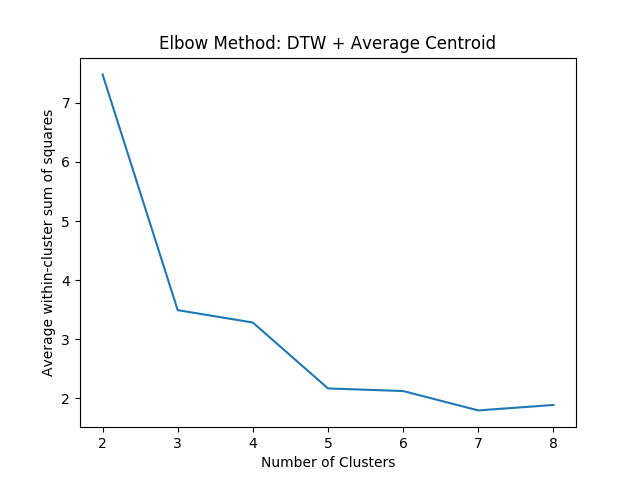
\includegraphics[scale=0.5]{images/raw_dtw_Average.png}
	\caption{Elbow method plot for the combination DTW + Average Centroid.}
	\label{elbow_method_euclidean}
\end{figure}

Results obtained with the Bary Center Averaging (DBA) method followed a similar trend with the main difference that a strong structure of the data is still suggested for k=3 clusters. Further raising the number of clusters lead to considerably low Silhouette Coefficient scores - ranging from about 0.32 all the way down to about 0.2. Such low values suggests a weak cluster structure.

When analysing the elbow plot - presented in Figure \ref{elbow_method_dba} - a steep drop can be seen when changing k from 3 to 4. If the number of clusters is further increased the average within-cluster sum of squares increases, which suggests a decrease in the cluster quality: samples in the same cluster are farther apart, meaning that clusters are less dense.

Based on the observations presented so far, a more careful analysis of the clusters obtained for $k = 3$ and $k = 4$ could be performed; however, an initial analysis of the centroids computed using this technique revealed inappropriate values in the context of water consumptions. Such findings suggest the inadequacy of this centroid computation method when applied to this particular problem and, therefore, a further study of clusters computed with this method will not be conducted.

\begin{figure}[ht]
	\centering
	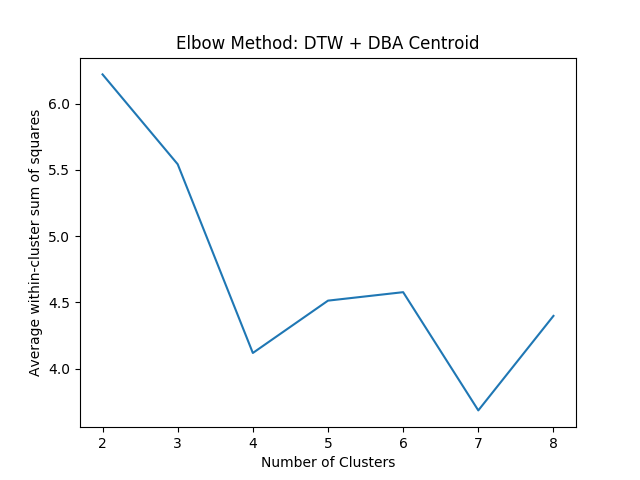
\includegraphics[scale=0.5]{images/raw_dtw_DBA.png}
	\caption{Elbow method plot for the combination DTW + DBA Centroid.}
	\label{elbow_method_dba}
\end{figure}

When the medoid method was instead used to compute the centroids (keeping DTW as the distance metric) the obtained results suggest a weak cluster structure in the data. In other words, the computed clusters do not appear to have adequate cluster properties: dense and well-separated. Besides scoring low silhouette coefficient scores - even for a small number of clusters such as 2 - the average within-cluster sum of squares remains constant, which is not a good indicator.

When dimensionality reduction techniques are applied - as in the case of \cite{abreu2012using} - obtained values for the silhouette coefficient appear to remain quite constant as the number of clusters is increased (ranging between about 0.52 and 0.60), which is a behaviour slightly different from the remainder situations.

Nevertheless, with the now common exception of the $k=2$ case, the mentioned SC values are not very high, suggesting only a reasonable cluster structure. By inspecting the elbow plot for this case (Figure \ref{elbow_method_euclidean_reduced}), a graphical analysis suggests that for $k = 5$ the decrease in the average within-cluster sum of squares is less steep, meaning that this could be a good target number of clusters with this approach.

\begin{figure}[ht]
	\centering
	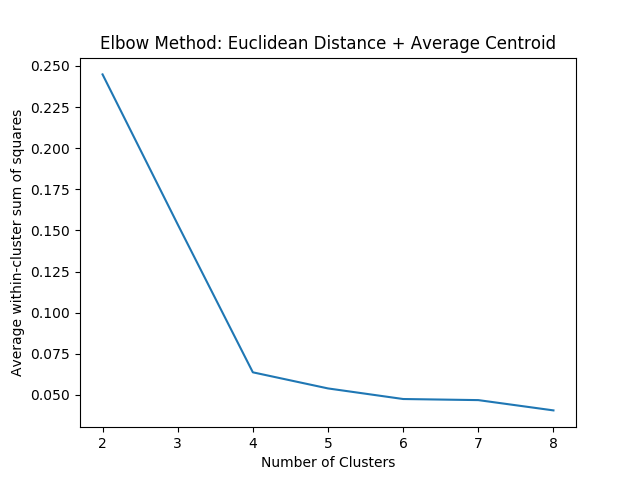
\includegraphics[scale=0.5]{images/reduced_euclidean_Average.png}
	\caption{Elbow method plot for the combination Euclidean Distance + Average Centroid.}
	\label{elbow_method_euclidean_reduced}
\end{figure}

The application of the TADPole clustering method produced, probably, the most unexpected results mostly due to the fact that an adequate cluster structure could only be achieved for 2 clusters. For all the other cases ($k = 3 - 8$) strongly inadequate cluster structures were determined, resulting in negative scores for the SC metric.

Another metric that supports the inferences suggested by the analysis of the silhouette scores is the Sum of Squared Errors: the highest values for this metric were registered with this approach. A similar scenario is observed for the Average Within-Cluster Sum of Squares.

Nevertheless, looking at the elbow plot in Figure \ref{elbow_method_tad} a sharp decrease in the average within-cluster sum of squares can be identified when increasing the number of clusters from 3 to 4. For higher numbers of clusters the plotted metric does not decrease as fast.

\begin{figure}[ht]
	\centering
	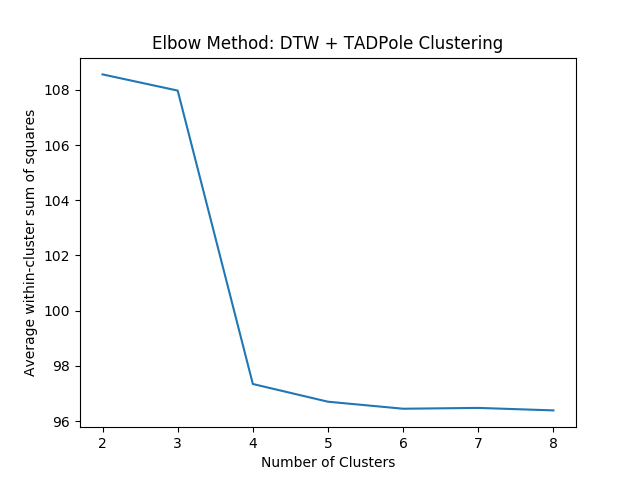
\includegraphics[scale=0.5]{images/raw_dtw_TADPole.png}
	\caption{Elbow method plot for the combination DTW + TADPole Clustering method.}
	\label{elbow_method_tad}
\end{figure}

\subsubsection{Remarks}

Generally, a decrease in the value of the SC metric was verified as the value of $k$ increased, which is an expected result. Indeed, for $k = 2$ the values of this metric tend to be high across all experiments, except when the medoid was used to compute the centroids (which produced very bad results for all values of $k$).

Performing a deeper and comparative analysis of the remainder metrics is not an easy task; as these are not limited metrics, its values can considerably change with different distance metrics and cluster centroid computation methods being adopted. Within the same combination of methods a comparison of the values of these metrics can be performed:

Regarding the Sum of Squared Errors, its value was expected to decrease as the number of clusters increased. This was only not verified for two scenarios, all for the K-Means algorithm: when the DTW distance and DBA centroid were combined (for $k = 4 - 6$ an increase was registered); and when the DTW distance and the medoid centroid were combined (values remained the same).

With respect to the Calinski-Herabaz coefficient, even though higher values suggest more dense and well-separated clusters, the increase in this metric was not always supported by an increase in the silhouette coefficient. This is the case for \emph{"dimensionality-reduced"} time series; application of the TADPole clustering algorithm and combination of the DTW with the medoid centroid computation method.

Based on these results, k=2 could be seen as good number of clusters in the sense that it produces well-separated and dense clusters (according to the SC metric). Nonetheless, two important aspects must be taken into account at this point:

First of all, as expected, when only two clusters are considered the errors (distance of each sample to its cluster centroid) are higher. Secondly, in the context of the problem being tackled, empiric knowledge suggests that more than 2 groups of similar consumption profiles can exist. Even though this is an intuition and not an established ground truth, the possibility of inspecting more than two clusters was chosen at this point. Future iterations of the current work could explore this alternative direction ($k = 2$).

In this sense a further results analysis will be performed on the following cases:

\begin{itemize}
	\item Application of the K-Means algorithm along with the euclidean distance metric and average centroid computation method for $k = 4$ and $k = 5$
	
	\item Application of the K-Means algorithm along with the DTW distance metric and average centroid computation method for $k = 4$ and $k = 5$
\end{itemize}

\subsection{Further Results Analysis}

The goal of the analysis conducted in the current section is to study in more detail water consumption patterns identified in the exercise detailed in previous sections. Such a task assumes an important role in unsupervised classification problems such as this one, mostly due to the difficulty in verifying if a given approach and/or solution is adequate and produces correct results for the problem being solved.

As such, the analysis performed at this point will focus on characterising the clusters identified in the scenarios presented at the end of the previous subsection.

Considering that the same ranges for the number of clusters were defined, different subsections will compose the remainder of the current section, each covering groupings with the same values of $k$\footnote{That is, with the same number of clusters.}.

\subsection{4 Clusters}

Figure \ref{centroids_4clusters} presents the centroids for the $4$ clusters computed in the two scenarios being considered.

\begin{figure*}
	\centering
	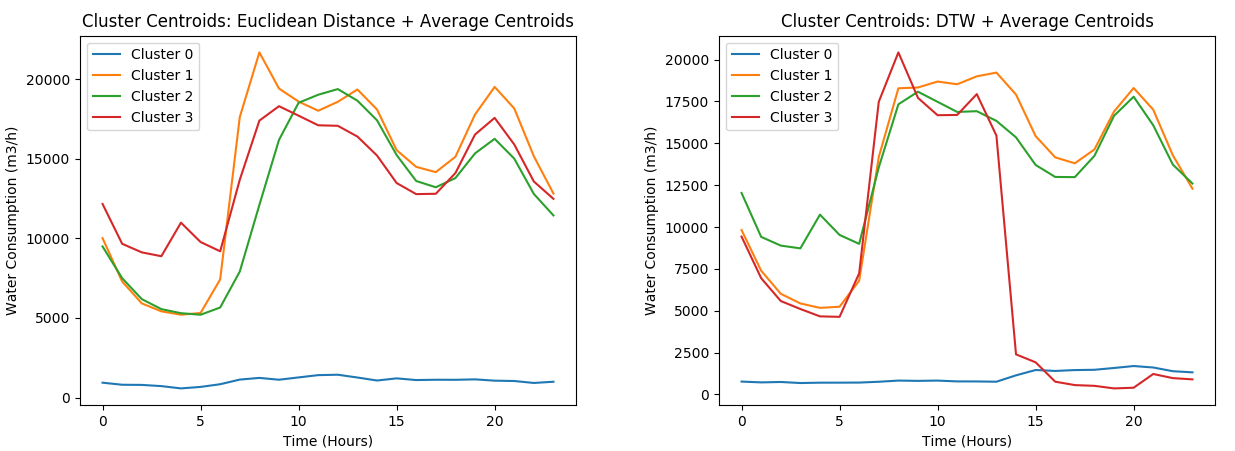
\includegraphics[scale=0.4]{images/centroids_4_clusters.png}
	\caption{Cluster centroids computed for a target number of clusters of $4$ with the K-Means algorithm along with the euclidean distance metric and average centroid computation method (a); and with the K-Means algorithm along with the DTW distance metric and average centroid computation method (b).}
	\label{centroids_4clusters}
\end{figure*}

\subsubsection{Residual Consumptions - Early Summer}
\label{residual_consumptions}

Immediately in both approaches there is one cluster that distinguishes itself from its siblings: in both cases it is \emph{Cluster 0}. Days whose consumptions belong in these clusters are characterised by residual water consumptions, which typically occur when buildings are unoccupied - during the holiday period or during weekends, if an industrial region is being studied (for example).

Further inspecting the composition of these clusters, it can be seen that not only the exact same number of days of the year are being assigned to them, but also the same percentage of weekdays and weekend-days and distribution over the months. Regarding this last point it can be seen that these low consumption profiles occur only during summer months (namely June and July).

Figures \ref{distribution_euclidean_average_4clusters} and \ref{distribution_raw_average_4clusters} support these statements.

\begin{figure*}
	\centering
	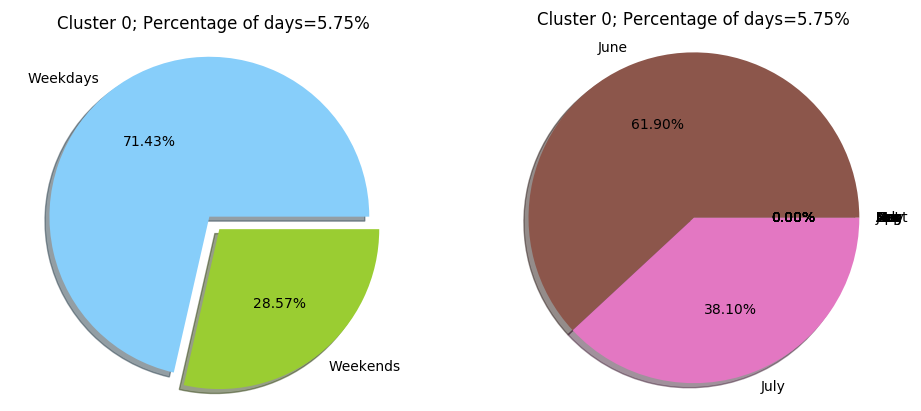
\includegraphics[scale=0.4]{images/percent_week_months_raw_average_4.png}
	\caption{Distribution of days over Cluster $0$ for the \emph{Euclidean Distance + Average Centroid} scenario: Percentage of weekdays and weekends (a) and distribution over months of the year (b).}
	\label{distribution_euclidean_average_4clusters}
\end{figure*}

\begin{figure*}
	\centering
	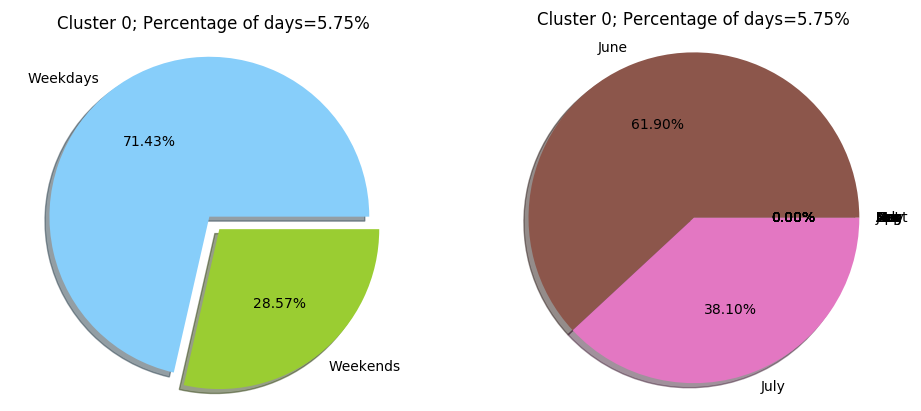
\includegraphics[scale=0.4]{images/percent_week_months_raw_average_4.png}
	\caption{Distribution of days over Cluster $0$ for the \emph{DTW + Average Centroid} scenario: Percentage of weekdays and weekends (a) and distribution over months of the year (b).}
	\label{distribution_raw_average_4clusters}
\end{figure*}

\subsubsection{Summer and Beginning of Autumn}

Observing Figure \ref{centroids_4clusters}, another similarity between clusters of both approaches can be identified, although it is not as clear as the previous one: cluster $3$ from Figure \ref{centroids_4clusters}a) - represented in red - and cluster $2$ from Figure \ref{centroids_4clusters}b) - represented in green - present consumption profiles with the same variations in the same moments of the day, and with roughly the same water consumptions.

Analysing their distribution of days over the year and percentages of weekdays and weekends, again similar distributions can be identified although they are not equal as in the previous case:

As seen in Figures \ref{cluster3_euclidean}b) and \ref{cluster2_raw}b), water consumptions that fall in the profiles represented by these clusters' centroids belong to part of the summer (July, August and part of September) and beginning of Autumn (end of September). A smaller percentage of days belonging to other seasons (namely the winter, in November) can also be identified in one of the approaches (Figure \ref{cluster2_raw}b), but has a very low incidence.

Water consumptions belonging to these periods are characterised by high demands during typical business hours: from about $7-8am$ to about $8pm$. It it also worth pointing out a slight decrease around $3pm$.

\begin{figure*}
	\centering
	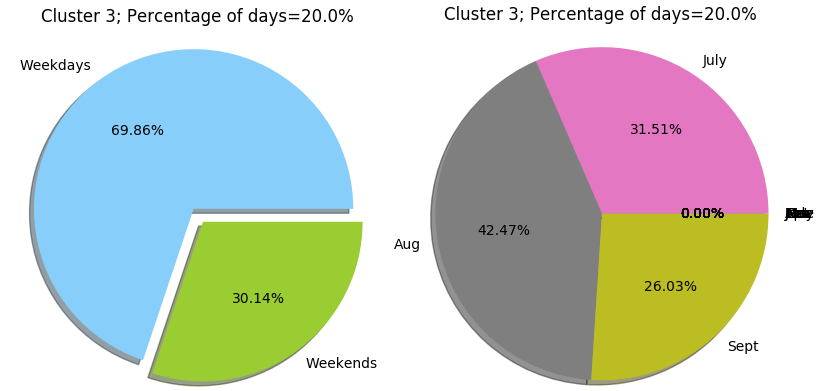
\includegraphics[scale=0.4]{images/percent_week__months_euc_average_cluster3_k4.png}
	\caption{Distribution of days over Cluster $3$ for the \emph{Euclidean Distance + Average Centroid} scenario: Percentage of weekdays and weekends (a) and distribution over months of the year (b).}
	\label{cluster3_euclidean}
\end{figure*}

Similarly to the previous case, weekends and weekdays appear to be evenly distributed in these clusters, taking into account their expected proportions: since a week is composed of $7$ days, $5$ of which are weekdays and only $2$ weekends, in this context, an even distribution of weekends and weekdays means that a proportion of about $70-30$ is registered.

Indeed, as supported by Figures \ref{cluster3_euclidean}a) and \ref{cluster2_raw}a), proportions between weekdays and weekends similar to this one have been verified.

\begin{figure*}
	\centering
	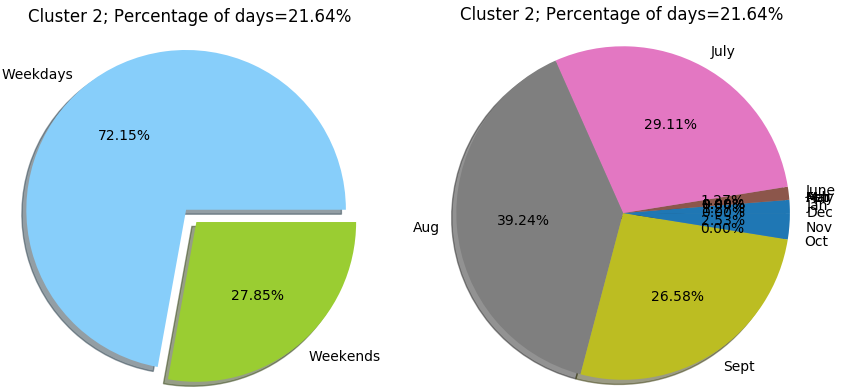
\includegraphics[scale=0.4]{images/percent_week_months_dtw_average_cluster2_k4.png}
	\caption{Distribution of days over Cluster $2$ for the \emph{DTW + Average Centroid} scenario: Percentage of weekdays and weekends (a) and distribution over months of the year (b).}
	\label{cluster2_raw}
\end{figure*}

\subsubsection{Entire Year}

In both approaches clusters that represent water consumption profiles that occur repeatedly throughout the year can also be identified, although similarities between clusters computed with both approaches might not be as clear as in previous cases.

Starting with the approach of Figure \ref{centroids_4clusters}a) - \emph{Euclidean} distance with \emph{Average} centroid method - clusters $1$ and $2$ are similar to a certain degree in terms of water consumptions and occurrence during the year, as suggested by Figure \ref{year_dist_k12_euc_average4}.

\begin{figure*}
	\centering
	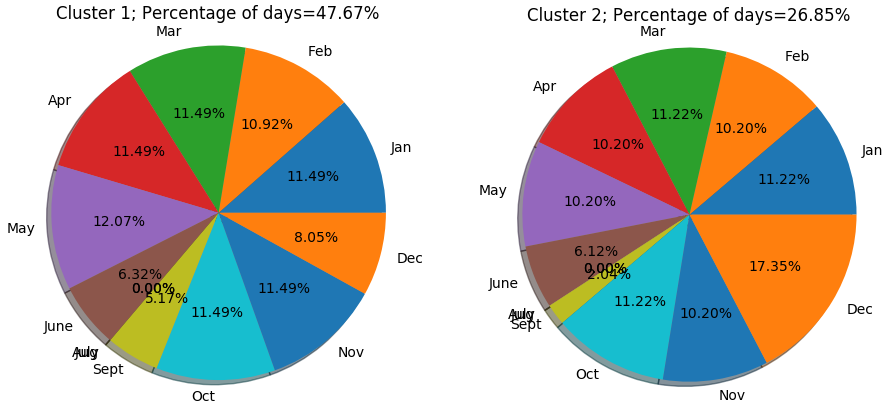
\includegraphics[scale=0.4]{images/percent_months_euc_average_k12_4.png}
	\caption{Distribution of days over the year for Clusters $1$ (a) and $2$ (b) for the \emph{Euclidean Distance + Average Centroid} scenario.}
	\label{year_dist_k12_euc_average4}
\end{figure*}

In terms of the water consumption profiles, the main difference between these two clusters is the overall higher consumptions of cluster $1$, specially during the early morning (between $8am$ and about $10am$) and the beginning of the night (around $8pm$).

Regarding distribution of days, as already mentioned both clusters have similar distribution over the year, containing identical percentages of days of each month of the year. Where these two clusters distinguish themselves from one another is in the distribution over the week: while cluster $1$ only contains weekdays, cluster $2$ is mainly composed of weekend days. Such statements are supported by the contents of Figure \ref{week_dist_k12_eu_average4}.

\begin{figure*}
	\centering
	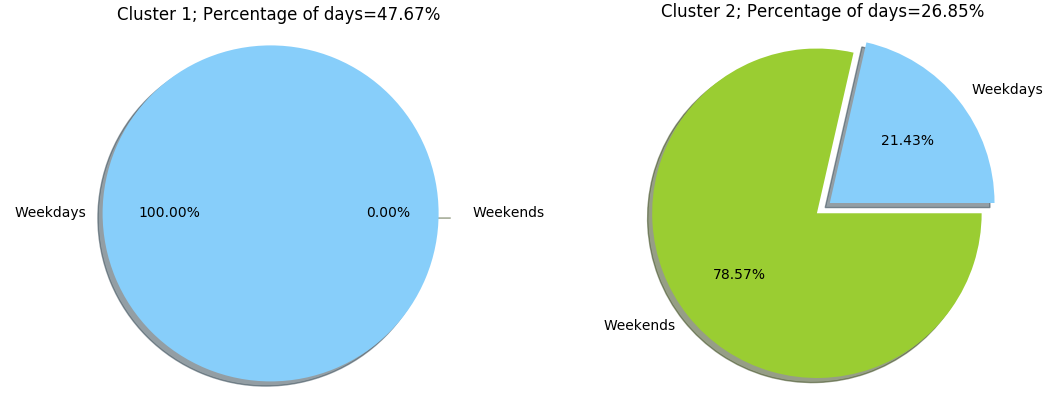
\includegraphics[scale=0.4]{images/percent_week_euc_average_k12_4.png}
	\caption{Distribution of days over the week for Clusters $1$ (a) and $2$ (b) for the \emph{Euclidean Distance + Average Centroid} scenario: Percentage of weekdays and weekends.}
	\label{week_dist_k12_eu_average4}
\end{figure*}

Moving on to the approach of Figure \ref{centroids_4clusters}b) - \emph{DTW} distance with \emph{Average} centroid method - cluster $1$ is also spread over the entire year. Of all the clusters computed in the two approaches being addressed in the current subsection, this cluster represents the highest percentage of the dataset ($72.6\%$).

When comparing this cluster with the two previously presented, besides the already mentioned similarities in the distribution over the year, equivalent percentages of the dataset are being represented: together, clusters $1$ and $2$ of \ref{centroids_4clusters}a) contain about $74.52\%$ of the days are being considered in this analysis.

Furthermore, similar distributions over the days of the week can be found, and in both cases they are close to the already mentioned expected ratio of $70-30$.

The main differences between these two groups - clusters $1$ and $2$ from \ref{centroids_4clusters}a) and cluster $1$ from \ref{centroids_4clusters}b) - are related with their water consumption profiles: a similar trend can be identified during early hours of the day (up until about $6am$) and after about $4pm$. In the mean time, cluster $1$ from \ref{centroids_4clusters}b) appears to characterise a more constant, and sometimes more intense, consumption profile.

All these statements are supported by the contents of Figure \ref{week_month_dist_k1_dtw_average4}.

\begin{figure*}
	\centering
	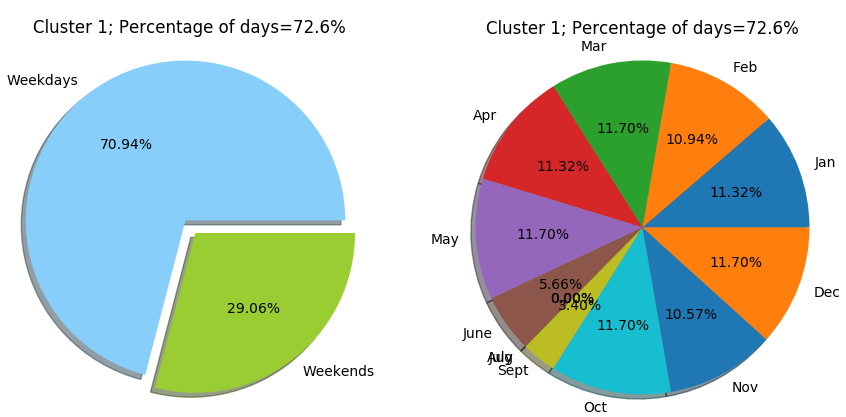
\includegraphics[scale=0.4]{images/percent_week_months_dtw_average_cluster1_k4.png}
	\caption{Distribution of days over Clusters $1$ for the \emph{DTW + Average Centroid} scenario: Percentage of weekdays and weekends (a) and distribution over the months of the year (b).}
	\label{week_month_dist_k1_dtw_average4}
\end{figure*}

\subsubsection{Isolated Clusters}
\label{isolated_clusters}

Finally, when performing K-Means Clustering with the DTW distance metric an isolated cluster can be identified: cluster $3$ contains only one day of the year during the month of June.

The fact that a unitary cluster has been identified does not, necessarily, signal any problem with the computed clusters: indeed, the Hierarchical Clustering initially performed and illustrated in Figure \ref{hierarchical_clustering_dtw} contains such clusters even for high cutoff distance values.

One possible reason that could lead to such a \emph{single-day} cluster has to do with the water consumption profile for this day: as presented in Figure \ref{centroids_4clusters}b), a sharp decrease in water consumptions during the afternoon and night can be observed, reaching consumptions even lower than the residual ones assigned to cluster $0$.

Nevertheless, it must be pointed out that this cluster has low representativeness, since it only contains one day with a clearly atypical consumption profile. 

\subsection{5 Clusters}
\label{5_clusters}

When considering one additional grouping computed clusters do not change drastically. Even though such a result could occur and depending on the data and clustering algorithms implemented even be justifiable, similar results to the ones presented in the previous subsection were expected.

This is, in fact, the case, as clusters representing similar consumption profiles were obtained at this point, and also featuring equivalent distributions over weekdays and throughout the entire year. As such, the discussion taking place in the current subsection will not follow the same organisation as the previous section: cluster solutions obtained with the same approach but for a different number of clusters will be compared; That is, cluster solutions obtained with \emph{Euclidean} distance and \emph{Average} centroid method for both $k=4$ and $k=5$ and cluster solutions obtained with \emph{DTW} distance and \emph{Average} centroid method for both $k=4$ and $k=5$ will be compared.

\subsubsection{Euclidean Distance and Average Centroid}

Overall, when dimensionality reduction techniques were applied no major differences in the computed water consumption profiles were registered when the target number of clusters was increased. Figure \ref{comparison_clusters_45_average} presents cluster centroids computed with both target number of clusters.

\begin{figure*}
	\centering
	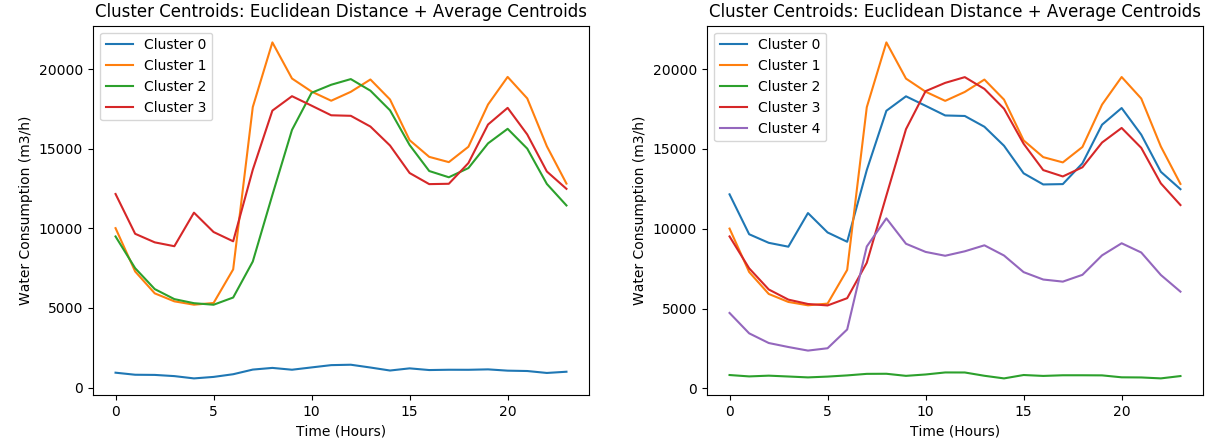
\includegraphics[scale=0.4]{images/centroids_45_clusters.png}
	\caption{Cluster centroids computed with the K-Means algorithm along with the \emph{Euclidean} distance metric and average centroid computation method for a target number of clusters of $4$ (a) and $5$ (b).}
	\label{comparison_clusters_45_average}
\end{figure*}

Analysing and comparing the distribution of days of the dataset throughout the clusters, equivalent compositions were found.

As already mentioned, one cluster representing residual consumptions during summer months can be found in both cases (Cluster $2$ for $k=5$), as well as one grouping representative of the terminal part of the summer (Cluster $0$ for $k=5$).

With respect to the typical consumption profiles that occur throughout the entire year (clusters $1$ and $2$ for $k=4$), almost the same consumption profiles and distribution of days were obtained with the new target number of clusters (clusters $1$ and $3$, respectively, for $k=5$).

Since one additional cluster must also be computed, cluster $4$ was also obtained; however, this cluster is not very representative, given the fact that only two days (one in June and another in July) were assigned to this cluster.

\subsubsection{DTW Distance and Average Centroid}

In the case in which clustering of raw time series data was performed, more visible changes in the computed consumption profiles were detected. Such a finding is mostly due to the disappearing of cluster $3$ which, has stated in \ref{isolated_clusters} has low representativeness.

Figure \ref{comparison_clusters_45_dtw} presents cluster centroids computed with both target number of clusters.

\begin{figure*}
	\centering
	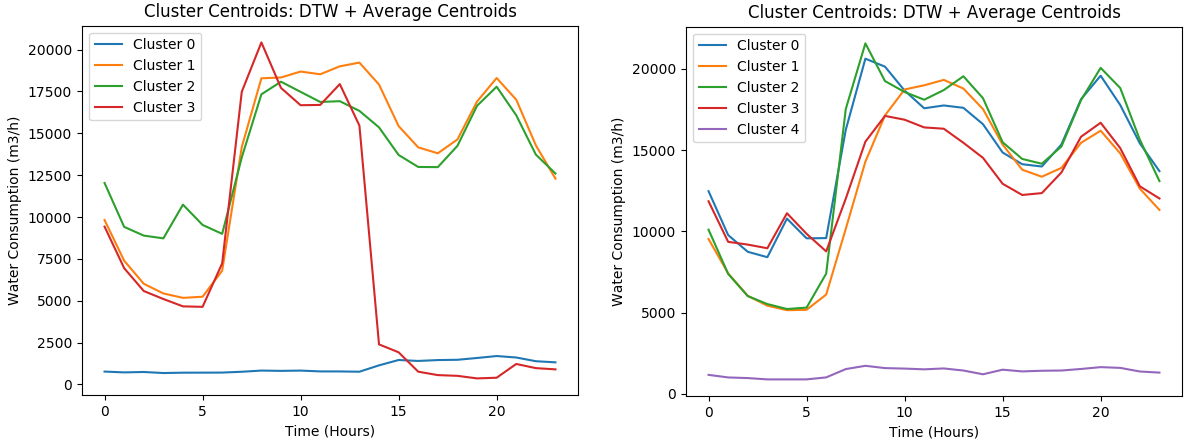
\includegraphics[scale=0.4]{images/centroids_45_clusters_dtw.png}
	\caption{Cluster centroids computed with the K-Means algorithm along with the \emph{DTW} distance metric and average centroid computation method for a target number of clusters of $4$ (a) and $5$ (b).}
	\label{comparison_clusters_45_dtw}
\end{figure*}

Analysing the plots in Figure \ref{comparison_clusters_45_dtw}, when increasing the number of clusters from $4$ to $5$ two distinct behaviours can be identified:

On the one hand, some cluster groupings remained almost the same, representing the same consumption profile over the day and containing the same distribution of days over the week and year. This is the case of the residual water consumptions: For $k=4$ cluster $0$ was representative of such behaviours and, for $k=5$, this is the job of cluster $4$. The only difference that must be referenced between the profiles represented by these two clusters is the fact that for $k=5$ water consumptions appear to increase earlier in the day (around $9am$) when in comparison with the cluster for $k=4$ (where water consumptions only increase around $2pm$).

On the other hand, some existing cluster groupings appear to have been split in two new clusters representing similar but slightly different consumption profiles. This is the case of cluster $1$ (which was split into clusters $0$ and $3$) and cluster $2$ (split into clusters $0$ and $3$). These new clusters maintain a similar distribution in terms of weekdays and days over the year.

With the mentioned cluster divisions resulting from the inclusion of an additional cluster, the number of elements assign to each cluster also suffers slight variations. For example, even though cluster $2$ was split into clusters $0$ and $3$, the total number of days in these two clusters is slightly inferior to the total number of days in the \emph{"original"} cluster $2$ (about $20.55\%$ of the dataset against approximately $21.64\%$).

If the number of elements in each cluster varies than so does the percentage of weekdays and weekends, and days of each month. Nevertheless, as in the situation described in the previous paragraph, these are slight variations, meaning that both the $4$ or $5$ identified groups represent a similar distribution and grouping of water consumptions.

\section{Conclusion}
\label{conclusions}

The current work studies methods and techniques for automatic categorisation of urban domestic water consumptions. Results not only show that such automatic categorisation is possible but also allow to pinpoint the periods during the year where certain consumption profiles occur.

Indeed, being able to recognise habitual water consumptions and to assign a time period to each characteristic, recurrent, consumption profile is of extreme importance to existing water companies, enabling them to manage their infrastructures more accurately and efficiently. 

As highlighted in Section \ref{methodology}, this work featured important steps that needed to be properly performed in order to allow for such automatic information categorisation. The lack of past experience with the produced data motivated a comparison of several methods in different moments of the execution. Such comparison was supported by a study of the literature in this topic, critic evaluation of results at any stage of the work and, sometimes, a \emph{trial-and-error} approach.

With respect to the actual categorisation of water consumptions several approaches were compared varying different parameters, of which the distance metric, clustering algorithm and centroid computation method are highlighted.

A somewhat preference was given to working with explicit time series data. Indeed, the main reasons for this choice were related with the popularity of this representation in time series clustering problems, as well as the existence of proper metrics to compare time series in such a representation. The main drawback of such a decision had to do with the high computational cost of working with explicit time series data (and of the adopted time series distance metric). As can be observed from the provided results and discussion, the application of alternative - and more \emph{traditional} - techniques enabled very similar results.

Another important decision that needed to be made was related with the evaluation of the computed solutions. In a completely unsupervised scenario such as this one, there is no way of accurately knowing which group of clusters (from a set of groupings proposed) represents more adequately recurrent behaviours in the dataset. Four cluster evaluation metrics were considered at this point in the work, with the \emph{Silhouette Coefficient} assuming a primary role.

The main reason for such a decision has to due with the fact that this is a metric for dense and well-separated clusters - characteristics that are always sought in this type of problem. Furthermore, this is the only limited metric; for all the others, values in different ranges may be obtained for distinct clustering algorithms, distance metrics, etc, strongly conditioning any attempt to compare cluster adequacy. Nevertheless, it should be pointed out that expert knowledge of the problem and data being processed is extremely important when analysing and evaluating clustering results.

Based on the results presented and the discussion conducted throughout the different sections that make up the document, the number of clusters (or number of recurrent water consumption profiles) that best fits the studied dataset appears to be $4$.

Certainly, as noted by the results presented in Section \ref{5_clusters}, increasing the number of clusters from $4$ to $5$ only lead to a separation of existing groupings, without leading to significative changes in the recurrent consumption profiles already identified. In addition, working with low dimensional time series data lead to similar groupings and similar consumption profiles\footnote{When in comparison with consumption profiles obtained with explicit time series data.}, at a considerably lower computational cost.

\section{Future Work}
\label{future_work}

Future iterations of the current work could and should study alternative paths to the one presented and followed.

For example, a considerably more extensive study on missing data imputation techniques could contribute towards the identification of methods more suited to provide estimations for missing data in this dataset and other datasets of the same nature.

In this line of though alternative representation techniques could also be employed, namely solutions that work with features extracted from the time series, such as average consumption, standard deviation, etc. Techniques of this nature would not only avoid producing estimates for missing values, but also reduce computational costs associated with the \emph{DTW} computation. A potential drawback of such solutions could be the lack of interpretability of the obtained results, as well as difficulties in obtaining a water consumption profile associated with each grouping.

Finally, even when working with explicit time series data, a discriminative analysis of the features (hours of the day in this case) that are responsible for assigning samples to a given cluster would also be valuable. Indeed, this would strongly contribute to a better understanding of the consumption profiles identified, and the hours of the day that are more important (and therefore critical) in each grouping.

\bibliographystyle{ieeetr}
\bibliography{bibliography.bib}

\end{document}